%  LaTeX support: latex@mdpi.com
%  In case you need support, please attach any log files that you could have, and specify the details of your LaTeX setup (which operating system and LaTeX version / tools you are using).

%=================================================================

% LaTeX Class File and Rendering Mode (choose one)
% You will need to save the "mdpi.cls" and "mdpi.bst" files into the same folder as this template file.

%=================================================================

\documentclass[journal,article,accept,moreauthors,pdftex,12pt,a4paper]{mdpi}
%--------------------
% Class Options:
%--------------------
% journal
%----------
% Choose between the following MDPI journals:
% actuators, administrativesciences, aerospace, agriculture, agronomy, algorithms, animals, antibiotics, antibodies, antioxidants, appliedsciences, arts, atmosphere, atoms, axioms, batteries, behavioralsciences, beverages, bioengineering, biology, biomedicines, biomimetics, biomolecules, biosensors, brainsciences, buildings, cancers, catalysts, cells, challenges, chemosensors, children, chromatography, climate, coatings, computation, computers, cosmetics, crystals, data, dentistryjournal, diagnostics, diseases, diversity, econometrics, economies, education, electronics, energies, entropy, environments, epigenomes, fermentation, fibers, foods, forests, futureinternet, galaxies, games, gels, genealogy, genes, geosciences, geriatrics, healthcare, horticulturae, humanities, hydrology, informatics, information, inorganics, insects, ijerph, ijfs, ijms, ijns, ijgi, jcdd, jcm, jdb, jfb, jfmk, jimaging, jof, joi, jlpea, jmse, jpm, jrfm, jsan, land, languages, laws, life, lubricants, machines, marinedrugs, materials, mathematics, medicalsciences, membranes, metabolites, metals, microarrays, micromachines, microorganisms, minerals, molbank, molecules, nanomaterials, ncrna, nutrients, pathogens, pharmaceuticals, pharmaceutics, pharmacy, philosophies, photonics, plants, polymers, processes, proteomes, publications, recycling, religions, remotesensing, resources, risks, robotics, safety, sensors, sinusitis, socialsciences, societies, sports, standards, sustainability, symmetry, systems, technologies, toxics, toxins, universe, vaccines, veterinarysciences, viruses, water
%---------
% article
%---------
% The default type of manuscript is article, but could be replaced by using one of the class options:
% article, review, communication, commentary, bookreview, correction, addendum, editorial, changes, supfile, casereport, comment, conceptpaper, conferencereport, meetingreport, discussion, essay, letter, newbookreceived, opinion, projectreport, reply, retraction, shortnote, technicalnote, creative, datadescriptor (for journal Data), briefreport, hypothesis, interestingimage
%----------
% submit
%----------
% The class option "submit" will be changed to "accept" by the Editorial Office when the paper is accepted. This will only make changes to the frontpage (e.g. the logo of the journal will get visible), the headings, and the copyright information. Journal info and pagination for accepted papers will also be assigned by the Editorial Office.
% Please insert a blank line is before and after all equation and eqnarray environments to ensure proper line numbering when option submit is chosen
%------------------
% moreauthors
%------------------
% If there is only one author the class option oneauthor should be used. Otherwise use the class option moreauthors.
%---------
% pdftex
%---------
% The option "pdftex" is for use with pdfLaTeX only. If eps figure are used, use the optioin "dvipdfm", with LaTeX and dvi2pdf only.

%=================================================================
\setcounter{page}{1}
\lastpage{x}
\doinum{10.3390/------}
\pubvolume{xx}
\pubyear{2015}
%\externaleditor{Academic Editor: xx}
\history{Received: xx / Accepted: xx / Published: xx}

\usepackage{dsfont}
\usepackage[utf8]{inputenc}
\usepackage{algorithm}
\usepackage{algorithmicx}
\usepackage{algpseudocode}

\newcommand{\xx}{\boldsymbol{x}}
\newcommand{\dx}{d\boldsymbol{x}}
\newcommand{\data}{\boldsymbol{D}}
\newcommand{\II}{\boldsymbol{I}}

%------------------------------------------------------------------
% The following line should be uncommented if the LaTeX file is uploaded to arXiv.org
%\pdfoutput=1

%=================================================================

% Add packages and commands to include here
% The amsmath, amsthm, amssymb, hyperref, caption, float and color packages are loaded by the MDPI class.
%\usepackage{graphicx}
%\usepackage{subfigure,psfig}

%=================================================================
%% Please use the following mathematics environments:
% \theoremstyle{mdpi}
% \newcounter{thm}
% \setcounter{thm}{0}
% \newcounter{ex}
% \setcounter{ex}{0}
% \newcounter{re}
% \setcounter{re}{0}
%
% \newtheorem{Theorem}[thm]{Theorem}
% \newtheorem{Lemma}[thm]{Lemma}
% \newtheorem{Corollary}[thm]{Corollary}
% \newtheorem{Proposition}[thm]{Proposition}
%
% \theoremstyle{mdpidefinition}
% \newtheorem{Characterization}[thm]{Characterization}
% \newtheorem{Property}[thm]{Property}
% \newtheorem{Problem}[thm]{Problem}
% \newtheorem{Example}[ex]{Example}
% \newtheorem{ExamplesandDefinitions}[ex]{Examples and Definitions}
% \newtheorem{Remark}[re]{Remark}
% \newtheorem{Definition}[thm]{Definition}
%% For proofs, please use the proof environment (the amsthm package is loaded by the MDPI class).

%=================================================================

% Full title of the paper (Capitalized)
\Title{Nested sampling with two objective functions}

% Authors (Add full first names)
\Author{Brendon J. Brewer$^{1,}$* and Ewan Cameron$^{2}$}

% Affiliations / Addresses (Add [1] after \address if there is only one affiliation.)
\address{%
$^{1}$ Department of Statistics, The University of Auckland, Private Bag 92019,
Auckland 1142, New Zealand\\
$^{2}$ Spatial Ecology and Epidemiology Group, Tinbergen Building, Department
of Zoology, University of Oxford, South Parks Road, Oxford, UK}

%\contributed{$^\dagger$ These authors contributed equally to this work.}

% Contact information of the corresponding author (Add [2] after \corres if there are more than one corresponding author.)
\corres{{\tt bj.brewer@auckland.ac.nz}}

% Abstract (Do not use inserted blank lines, i.e. \\)
\abstract{We present a generalization of the Nested Sampling algorithm to a
broad class of problems which arise in statistical mechanics.}

% Keywords: add 3 to 10 keywords
\keyword{nested sampling; bayesian computation; statistical mechanics}

% The fields PACS, MSC, and JEL may be left empty or commented out if not applicable
%\PACS{}
%\MSC{}
%\JEL{}

% If this is an expanded version of a conference paper, please cite it here: enter the full citation of your conference paper, and add $^\dagger$ in the end of the title of this article.
%\conference{}

%%%%%%%%%%%%%%%%%%%%%%%%%%%%%%%%%%%%%%%%%%
% For journal Data:

%\dataset{DOI number or link to the deposited data set in cases where the data set is published or set to be published separately. If the data set is submitted and will be published as a supplement to this paper in the journal Data, this field will be filled by the editors of the journal. In this case, please make sure to submit the data set as a supplement when entering your manuscript into our manuscript editorial system.}
%\datasetlicense{license under which the data set is made available (CC0, CC-BY, CC-BY-SA, CC-BY-NC, etc.)}

%%%%%%%%%%%%%%%%%%%%%%%%%%%%%%%%%%%%%%%%%%

\begin{document}

%%%%%%%%%%%%%%%%%%%%%%%%%%%%%%%%%%%%%%%%%%

\section{Introduction}

Nested Sampling \citep[NS][]{skilling} is an effective and popular
Monte Carlo algorithm which can solve a wide range of problems in Bayesian
computation and statistical mechanics
\citep{2009arXiv0906.3544P, 2014PhRvE..89b2302P, 2015arXiv150303404B}.
In a Bayesian inference problem with unknown parameters denoted collectively
by a vector $\xx$, the
posterior distribution for the parameters given data $\data$ (and prior
information $\II$) is:
\begin{eqnarray}
p(\xx | \data, \II) &=&
\frac{p(\xx | \II)p(\data | \xx, \II)}{p(\data | \II)}\\
&=& \frac{\pi(\xx)L(\xx)}{Z}
\end{eqnarray}
where $\pi(\xx)$ is the prior distribution, $L(\xx)$ is the likelihood
function, and $Z$ is the normalising constant, usually known as the
``marginal likelihood'' or the ``evidence'':
\begin{eqnarray}
Z &=& \int \pi(\xx) L(\xx) \, \dx.\label{eqn:evidence}
\end{eqnarray}
NS begins by drawing particles from the
prior $\pi(\xx)$ and successively imposing constraints on the value of
the likelihood $L(\xx)$ that compress the prior mass by an
approximately-known factor. Like other related algorithms such as those
based on ``annealing'', NS
moves through a sequence of probability distributions beginning from the
prior. This sequence of distributions is defined by
\begin{eqnarray}
p(\xx; \ell) &=& \frac{1}{X(\ell)}\pi(\xx)\mathds{1}\left(L(\xx) > \ell\right).
\end{eqnarray}

This enables the calculation of the marginal likelihood $Z$
and properties of the posterior $\pi(\xx)L(\xx)/Z$.
NS is required because Equation~\ref{eqn:evidence}
is the expected value of $L$ with respect to a very heavy-tailed distribution
(the prior for the $L$ value implied by $\pi(\xx)$). Hence, there is a strong
connection between NS and ideas from rare event simulation \citep{walter}.

NS also allows us to calculate the properties of any other distribution that
is in some sense intermediate
between the prior and the posterior. For example, we might be interested in
a ``power posterior'' where the likelihood is raised to a power $\beta$:
\begin{eqnarray}
p(\xx; \beta) &=& \frac{\pi(\xx)L(\xx)^\beta}{Z(\beta)}\label{eqn:power_posterior}
\end{eqnarray}
The normalisation and posterior samples from this distribution can be obtained
from the original NS run by re-weighting the output according to $L(\xx)^\beta$
instead of the usual $L(\xx)$ used to obtain the posterior.
An example application, in the case of
a Bayesian inference problem with a ``gaussian noise'' likelihood assumption,
computing $p(\xx; \beta)$ for $\beta \neq 1$ allows us to explore what the
posterior distribution would have been if the noise variance had been greater.
This is different from including an extra parameter to allow the noise variance
to be greater, because NS allows you to test the consequences of values of the
variance that are very implausible given the data.

Alternatives to NS include methods based on ``annealing'', where a sequence of
distributions of the form of Equation~\ref{eqn:power_posterior} is used.
There are many different methods based on this idea, such as the popular
parallel tempering method \citep{pt}.
However, unlike annealing methods, NS continues
to work when the problem contains a phase transition.

In statistical mechanics, Equation~\ref{eqn:power_posterior} defines the
family of {\it canonical distributions}, usually written as:
\begin{eqnarray}
p(\xx; \beta) &=& \frac{\pi(\xx)\exp[-\beta E(\xx)]}{Z(\beta)}
\end{eqnarray}
where $E(\xx)$ is the energy function, and $\pi(\xx)$ is often uniform over
phase space (the set of possible positions and momenta of a collection of
particles) or configuration space (the set of possible positions of a collection
of particles). In this context we usually want to
compute $Z(\beta)$ as a function of $\beta$, which is called the
{\it partition function}. NS can achieve this, allowing the study of
the properties of materials from first principles, based on hypotheses about
the atoms or molecules that make them up \citep[e.g.][]{2009arXiv0906.3544P,
2014PhRvE..89b2302P, 2015arXiv150303404B}.

In some inference and
statistical mechanics problems, there are two or more scalar functions of
$\xx$ that are relevant. Suppose our prior is $\pi(\xx)$ as before, and
we obtain testable information that fixes the expected values of two scalar
functions of $\xx$, $L_1(\xx)$ and $L_2(\xx)$. It is well known that the
updated probability distribution that takes into account the constraints is
of the ``canonical'' form:

\begin{eqnarray}
p(\xx; \beta_1, \beta_2) &=& \frac{\pi(\xx)\exp\left[\beta_1L_1(\xx)+\beta_2L_2(\xx)\right]}
{Z(\beta_1, \beta_2)}
\end{eqnarray}

If we were only interested in a single canonical distribution, for example
with $\beta_1 = 0.3$ and $\beta_2 = 0.7$, we could estimate its normalising
constant and by running standard Nested Sampling with ``likelihood''
$L(\xx) = \exp\left[0.3L_1(\xx) + 0.7L_2(\xx)\right]$. However, usually we
are interested in a range of values for $\beta_1$ and $\beta_2$, and we
want to know the normalisation $Z(\beta_1, \beta_2)$, called the
partition function. This work describes
progress towards solving this class of problems while maintaining the benefits
of Nested Sampling, such as the ability to cope with first-order phase
transitions. The algorithm is designed for problems with two objective
functions, but should generalize to problems with more than two (though perhaps
not more than a few).

The prior $\pi(\xx)$ implies a certain prior for $L_1$ and $L_2$, which we
denote $\pi(L_1, L_2)$. An example of a prior is shown as the
probability density in Figure~\ref{fig:joint1}. The partition function
$Z(\beta_1, \beta_2)$ is a set of expected values with respect to this density.
Simple Monte Carlo sampling from $\pi$ will not work except for values of
$(\beta_1, \beta_2)$ where the canonical distribution remains similar to $\pi$.
We need a sampler that explores regions where $L_1$ and $L_2$ are high in order
to accurately estimate $Z(\beta_1, \beta_2)$.

\begin{figure}
\centering
\includegraphics[scale=0.5]{figures/joint1.pdf}
\caption{\it An example of a prior for $L_1$ and $L_2$, which is implied by
the prior $\pi(\xx)$. We have overplotted some points drawn from this prior.
\label{fig:joint1}}
\end{figure}

Our proposed algorithm (introduced in Section~\ref{sec:algorithm}) makes use
of a quantity we call the corner count. For any values $(\ell_1, \ell_2)$,
the prior mass for which both objective functions are lower is
\begin{eqnarray}
X(\ell_1, \ell_2) &=& \int \pi(L_1, L_2) \mathds{1}\left(L_1 < \ell_1, L_2 < \ell_2 \right)
 \, dL_1 \, dL_2
\end{eqnarray}
This is the two dimensional cumulative distribution function (CDF) of
$L_1$ and $L_2$.


The corner count of particle $i$ is defined as the number of particles with
a lower value of {\em both} objective functions compared to particle $i$.
Graphically, on a plot of $L_2$ vs. $L_1$ the corner count is the number of
particles in the rectangle whose upper right corner is at
$\left(L_1(\xx_i), L_2(\xx_i)\right)$ (see Figure~\ref{fig:joint2} for an
example). The equation for the corner count is:
\begin{eqnarray}
C_i &=& \sum_{j=1}^N \mathds{1}\left(L_1(\xx_j) < L_1(\xx_i),
L_2(\xx_j) < L_2(\xx_i)
\right).\label{eqn:corner_count}
\end{eqnarray}


\section{Properties of Nested sampling}

We seek an algorithm for computing the partition function
$Z(\beta_1, \beta_2)$ for a range of values of the $\beta$s, from a single
run. To be considered a variant of Nested Sampling, the method should satisfy
the following properties:
\begin{enumerate}
\item The algorithm should begin with $N$ points drawn from the prior $\pi(\xx)$.
\item The algorithm should seek to explore regions where the values of
$L_1(\xx)$ and $L_2(\xx)$ are greater than what would be expected from the
prior.
\item The algorithm should consider a sequence of probability
distributions proportional to $\pi$, but restricted to smaller and smaller
domains for which we can approximately measure the enclosed prior mass.
\item The algorithm should be invariant to monotonic transformations of
$L_1$ and $L_2$, i.e. it should only depend on rankings of $L_1$ and $L_2$
values and not the values themselves.
\end{enumerate}


\begin{figure}
\centering
\includegraphics[scale=0.5]{figures/joint2.pdf}
\caption{\it The same as Figure~\ref{fig:joint1}.
\label{fig:joint2}}
\end{figure}



\section{Proposed algorithm}\label{sec:algorithm}

Here we describe the proposed algorithm, which took three years of
experimentation to develop. Please contact the first author for a list of
failed ideas, some of which might lead to potential alternatives to this
algorithm. 

\begin{algorithm}
\begin{algorithmic}
\State Generate $N$ particles $\{\xx_1, ..., \xx_N\}$ from $\pi(\xx)$.
\While{more iterations desired}
	\State Calculate the {\it corner count} (Equation~\ref{eqn:corner_count})
of each particle.
	\State Choose one of the particles which has corner count equal to the
minimum nonzero value. If all particles have a corner count of zero,
the algorithm terminates. Call the selected particle particle $K$.
	\State Choose one of the objective functions, and find $K$'s rank in terms
of that objective function.
\EndWhile
\end{algorithmic}
\end{algorithm}

Step 1 of the algorithm ensures that NS property 1 is trivially satisfied.



\section{Test problem}

We tested the algorithm on a simple 100-dimensional example, where the
prior is a uniform distribution between 0 and 1 for each coordinate:
\begin{eqnarray}
\pi(\xx) &=& \prod_{i=1}^{100}
\left\{
\begin{array}{lr}
1, & x_i \in [0, 1]\\
0, & \textnormal{otherwise.}
\end{array}
\right.
\end{eqnarray}
The two objective functions are:
\begin{eqnarray}
L_1(\xx) &=& -\sum_{i=1}^{100} \left(x_i - 0.5\right)^2\\
L_2(\xx) &=& -\sum_{i=1}^{100} \log\left[1 +
\left(\frac{x_i - 0.5}{0.01}\right)^2
\right].
\end{eqnarray}
The canonical distribution at low temperature for $L_1$ and high temperature
for $L_2$ is a gaussian centered at 0.5 with standard deviation
$\sqrt{T_1/2}$. At high temperatures for $L_2$ and low temperatures for $L_1$ the
canonical distributions are Cauchy centered at 0.5 with width
$0.01\sqrt{T_2}$.

\begin{figure}
\centering
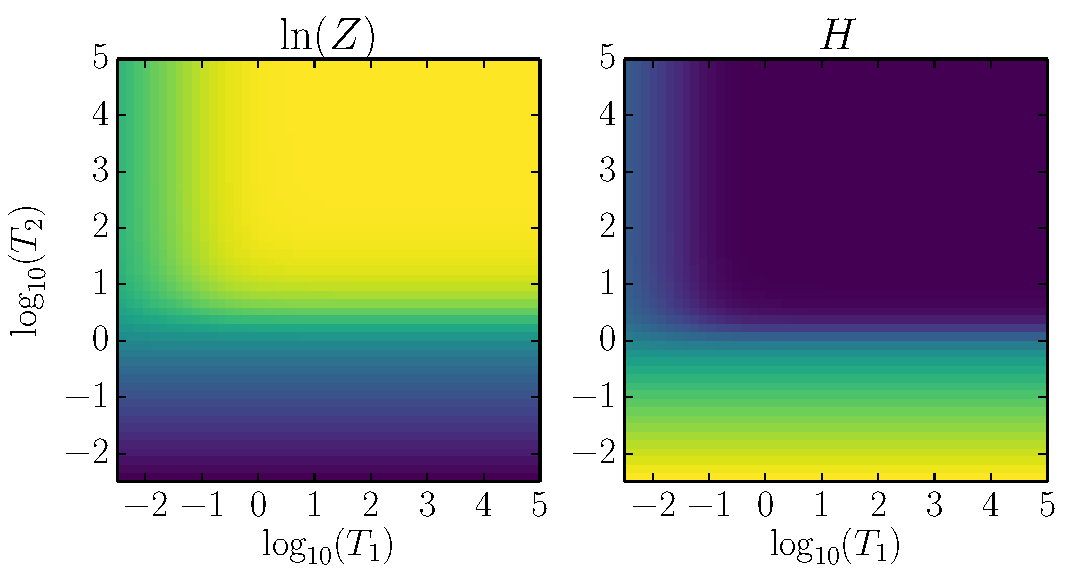
\includegraphics[scale=0.75]{figures/truth.pdf}
\caption{\label{fig:truth}}
\end{figure}


\begin{figure}
\centering
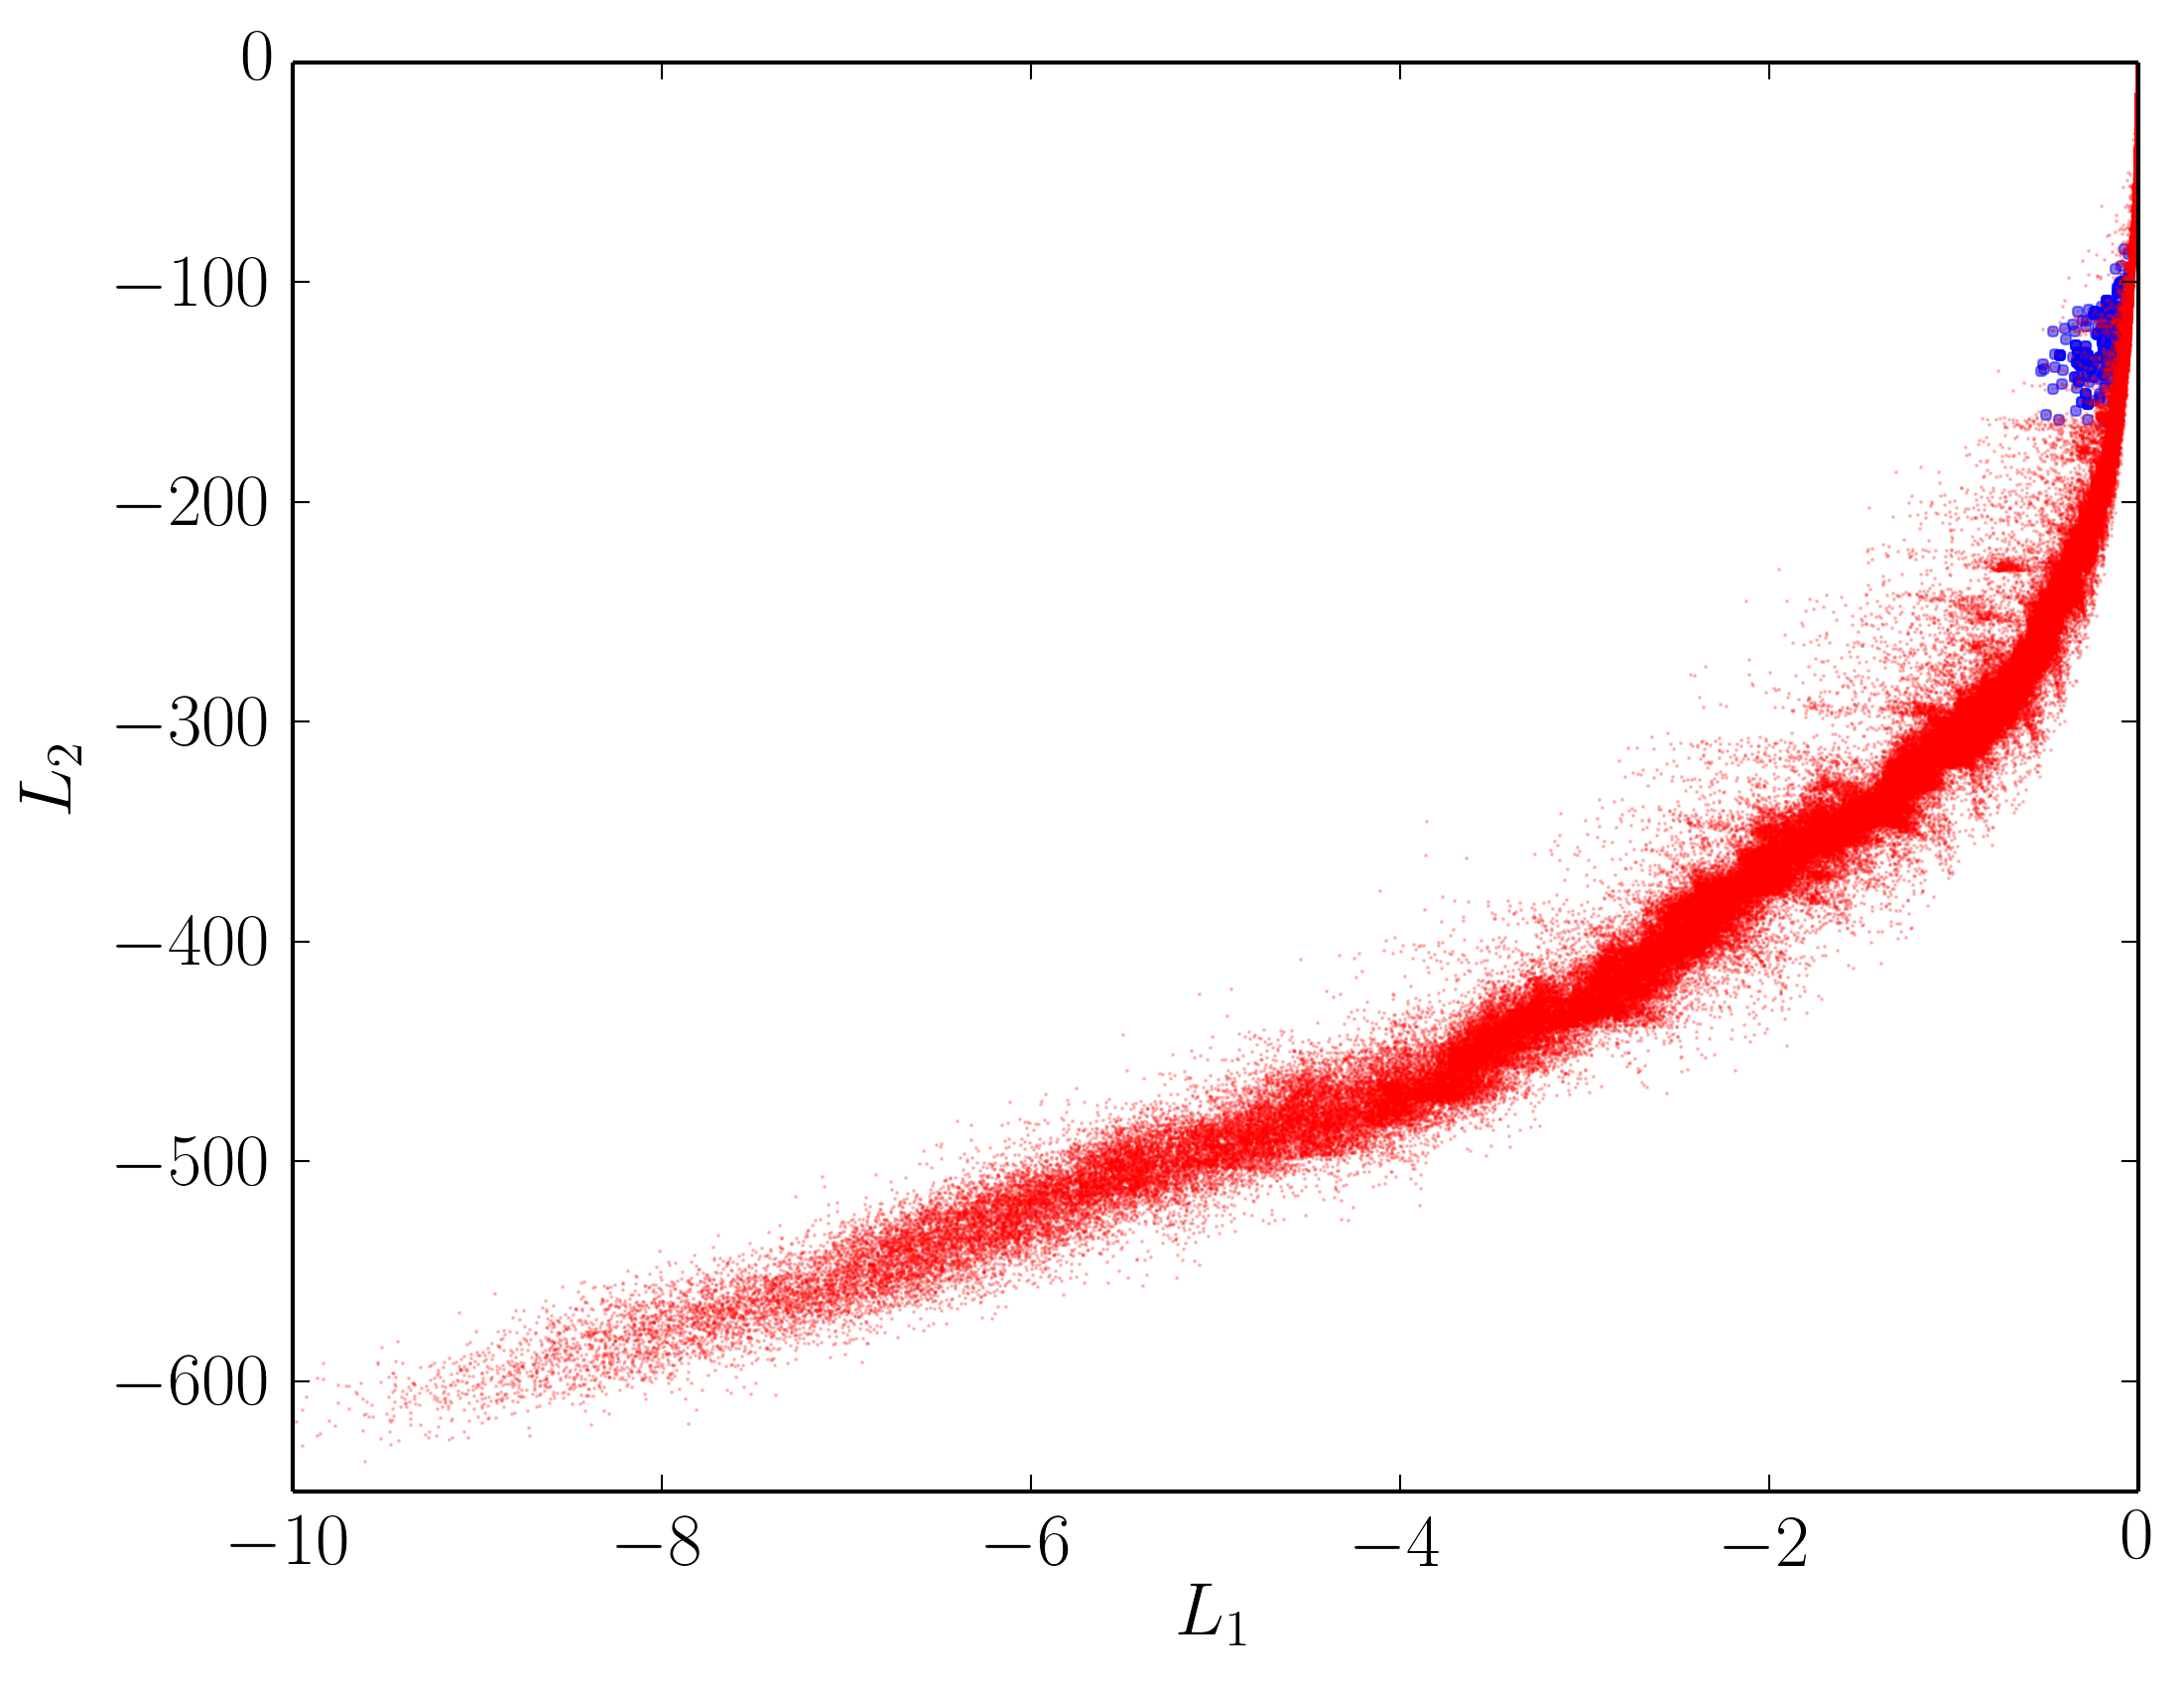
\includegraphics[scale=0.75]{figures/output.png}
\caption{\label{fig:output}}
\end{figure}



\begin{figure}
\centering
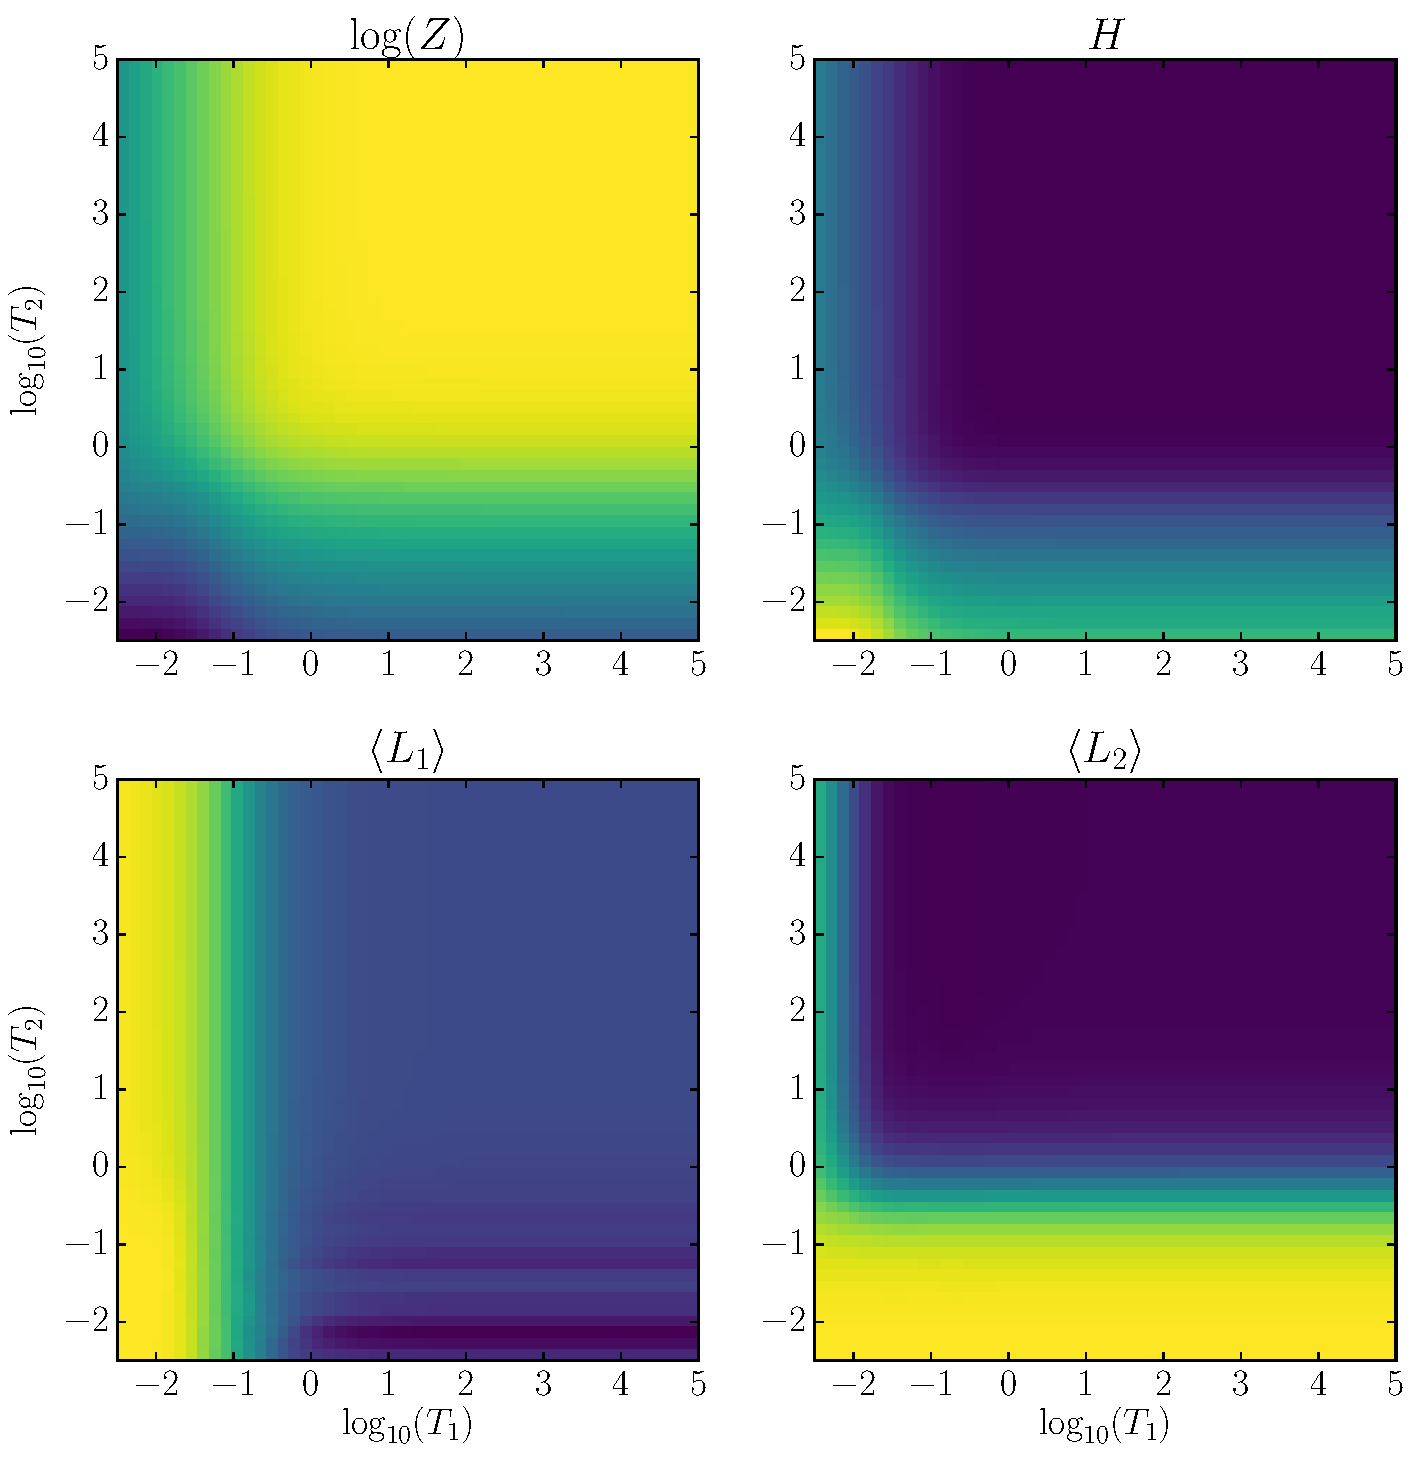
\includegraphics[scale=0.5]{figures/results.pdf}
\caption{Numerical results for the test problem. These compare well with the
true partition function and KL divergence given in Figure~\ref{fig:truth}.
\label{fig:results}}
\end{figure}


\section{What kind of accuracy can we expect?}

Imagine computing $Z(\beta_1, \beta_2)$ by looping over a grid of $\beta_2$
values and doing an NS run with respect to $L_1$ for each. For each
value of $\beta_1$ and $\beta_2$ that we're interested in, we can expect
a (marginal) ``one-sigma'' accuracy in
$\ln\left[Z(\beta_1, \beta_2)\right]$ of $\pm \sqrt{H(\beta_1, \beta_2)/N}$,
for a computational cost proportional to...

\section{What kind of accuracy do we need?}

The following argument is due to John Skilling. Consider Bayesian model selection
between two models $M_1$ and $M_2$. The Bayes Factor is the ratio of the
two marginal likelihoods:
\begin{eqnarray}
B = \frac{P(D | M_1)}{P(D | M_2)} = \frac{Z_1}{Z_2}
\end{eqnarray}
In large problems, the log of the Bayes Factor is usually more convenient:
\begin{eqnarray}
\ln B = \ln Z_1 - \ln Z_2.
\end{eqnarray}
Naively, we want $\ln B$ to an accuracy of about 0.1, so that we can reliably
quantify the strength of the evidence when the two models are similarly
supported by the data. But is this a realistic situation?
Prior to the data, we don't know the
value of $\ln B$. Rather, $\ln B$ has a prior distribution. We can find this
prior in terms of its CDF:
\begin{eqnarray}
P(\ln B \leq R) &=& \int P(D)P(\ln B \leq R | D) \, dD\\
&=& \int P(D) \mathds{1}\left(\ln B(D) \leq R\right) \, dD\\
&=& \int \sum_{i\in\{1,2\}}\left[P(M_i)P(D|M_i)\right] \mathds{1}\left(\ln B(D) \leq R\right) \, dD
\end{eqnarray}



%Use Skilling's argument about the prior distribution of a log Bayes factor.
%Even though the performance of this algorithm won't be great for high $H$, it
%will be good enough. I think the probability it won't give enough accuracy will
%be ``exponentially small''.

\acknowledgments{Acknowledgements}

It is a pleasure to thank Gábor Csányi (Cambridge), Livia B. Pártay (Cambridge),
and Robert Baldock (Cambridge) for valuable conversations.

%%%%%%%%%%%%%%%%%%%%%%%%%%%%%%%%%%%%%%%%%%

\authorcontributions{Author Contributions}

Required if more than one author. Authorship must include and be strictly limited to researchers who have substantially contributed to the reported work. Please carefully review our criteria regarding the Qualification for Authorship: \web /instructions.

%%%%%%%%%%%%%%%%%%%%%%%%%%%%%%%%%%%%%%%%%%

\conflictofinterests{Conflicts of Interest}
The authors declare no conflict of interest.

%=================================================================
% References: Variant A
%=================================================================
% Back Matter (References and Notes)
%----------------------------------------------------------
% Style and layout of the references
\bibliographystyle{mdpi}
\makeatletter
\renewcommand\@biblabel[1]{#1. }
\makeatother

\begin{thebibliography}{999} % if there are less than 10 entries, enter a one digit number

\bibitem[Baldock et al.(2015)]{2015arXiv150303404B} Baldock, R.~J.~N., 
P{\'a}rtay, L.~v.~B., Bart{\'o}k, A.~P., Payne, M.~C., Cs{\'a}nyi, G.\ 
2015.\ Determining pressure-temperature phase diagrams of materials.\ ArXiv 
e-prints arXiv: 1503.03404. 

\bibitem[Hansmann(1997)]{pt} Hansmann, Ulrich HE., 1997, ``Parallel tempering algorithm for conformational studies of biological molecules.'', Chemical Physics Letters 281, no. 1 (1997): 140-150.

\bibitem[P{\'a}rtay et al.(2014)]{2014PhRvE..89b2302P} P{\'a}rtay, L.~B., 
Bart{\'o}k, A.~P., Cs{\'a}nyi, G.\ 2014.\ Nested sampling for materials: 
The case of hard spheres.\ Physical Review E 89, 022302. 

\bibitem[P{\'a}rtay et al.(2009)]{2009arXiv0906.3544P} P{\'a}rtay, L.~B., 
Bart{\'o}k, A.~P., Cs{\'a}nyi, G.\ 2009.\ Efficient sampling of atomic 
configurational spaces.\ ArXiv e-prints arXiv: 0906.3544. 

\bibitem[\protect\citeauthoryear{Skilling}{2006}]{skilling} Skilling, J., 2006, Nested Sampling for General Bayesian Computation, Bayesian Analysis 4, pp. 833-860.

\bibitem[Walter(2015)]{walter}
Walter, C.\ Point Process-based Monte Carlo estimation.\ arXiv: 1412.6368.
%% Reference 1
%\bibitem{ref-journal}
%Lastname, F.; Author, T. The title of the cited article. {\em Journal Abbreviation} {\bf 2008}, {\em 10}, 142-149.

%% Reference 2
%\bibitem{ref-book}
%Lastname, F.F.; Author, T. The title of the cited contribution. In {\em The Book Title}; Editor, F., Meditor, A., Eds.; Publishing House: City, Country, 2007; pp. 32-58.

\end{thebibliography}

%=================================================================
% References:  Variant B
%=================================================================
% Use the following option to include external BibTeX files:
%\bibliography{lite}
%\bibliographystyle{mdpi}

%%%%%%%%%%%%%%%%%%%%%%%%%%%%%%%%%%%%%%%%%%

%\abbreviations{Abbreviations/Nomenclature}
%
%Main text.

%%%%%%%%%%%%%%%%%%%%%%%%%%%%%%%%%%%%%%%%%%

%\appendix
%\section{Appendix Title}
%
%Main text.

\end{document}

